\documentclass[letter,10pt]{article}

\usepackage[tagged]{accessibility}

\usepackage[margin=1cm,landscape]{geometry}

\usepackage{multicol}
\usepackage{tikz,lipsum,lmodern}
\usepackage[most]{tcolorbox}

\PassOptionsToPackage{hyphens}{url}
\usepackage[hidelinks]{hyperref}

\usepackage{booktabs,siunitx}
\usepackage{breakurl}

% \usepackage[table]{xcolor} 
\usepackage{fancyvrb}
\usepackage{listings}
\usepackage{xcolor}
\usepackage{tikz}
\usepackage{forest}
\usepackage{adjustbox}
\usetikzlibrary{arrows.meta,shadows}
\usepackage{array,multirow,graphicx}
\setcounter{tocdepth}{9}
\usepackage{enumitem} 
%\providecommand{\tightlist}{%
%  \setlength{\itemsep}{0pt}\setlength{\parskip}{0pt}}

\newcommand{\TODO}[1]{\todo[inline]{#1}}

\newcommand{\RULE}{\hrule
\vspace{1pt}
\hrule height 1pt
}

\newcommand{\ngreen}{bottom color=green!20}
\newcommand{\ngrey}{bottom color=gray!20}
\newcommand{\nred}{bottom color=red!20}
\newcommand{\nwhite}{bottom color=white!20}

\newcommand{\Figure}[1]{Fig.~\ref{#1}}
\newcommand{\Section}[1]{Sec.~\ref{#1}}
\newcommand{\Table}[1]{Tab.~\ref{#1}}

\newcommand{\TwoFIGURES}[6]{
\begin{figure}[htb]
\centering

\includegraphics[width=\columnwidth]{images/#1}

\caption{#2}
\label{#3}

\centering

\includegraphics[width=\columnwidth]{images/#4}

\caption{#5}
\label{#6}
\end{figure}
}

\newcommand{\OneFIGURE}[3]{
\begin{figure}[htb]
\centering

\includegraphics[width=\columnwidth]{images/#1}

\caption{#2}
\label{#3}

\end{figure}
}

\newcommand{\ExternalLink}{%
    \tikz[x=1.2ex, y=1.2ex, baseline=-0.05ex]{% 
        \begin{scope}[x=1ex, y=1ex]
            \clip (-0.1,-0.1) 
                --++ (-0, 1.2) 
                --++ (0.6, 0) 
                --++ (0, -0.6) 
                --++ (0.6, 0) 
                --++ (0, -1);
            \path[draw, 
                line width = 0.5, 
                rounded corners=0.5] 
                (0,0) rectangle (1,1);
        \end{scope}
        \path[draw, line width = 0.5] (0.5, 0.5) 
            -- (1, 1);
        \path[draw, line width = 0.5] (0.6, 1) 
            -- (1, 1) -- (1, 0.6);
        }
    }

\newcommand{\Link}[1]{\href{#1}{\ExternalLink}}


\usepackage{pdfcomment}
\usepackage[explicit]{titlesec}
\usepackage[normalem]{ulem}

\setlength{\columnseprule}{0.4pt}
\date{}

\hypersetup{
    pdfauthor={Gregor von Laszewski,
               Anthony Orlowski,
               Richard Otten,
               Adam Chai,
               Reilly Markowitz,
               Sunny Gandhi,
               Caleb Wilson},
    pdfsubject={UROC},
    pdftitle={Towards Automatically Generated Hybrid Multi-Cloud AI Services},
    pdfkeywords={multi-cloud, hybrid cloud, AI services, REST, cloudmesh}
}

\begin{document}

\vspace{-3.5cm}


\begin{figure}[!h]
\begin{tcolorbox}[enhanced,
  frame style,
  colback=red!10,
  colframe=red!75!black]

{\Large\bf Towards Automatically Generated Hybrid Multi-Cloud AI Services} 


{\em Gregor von Laszewski,
Anthony Orlowski,
Richard Otten,
Adam Chai$*$,
Reilly Markowitz$*$,
Sunny Gandhi$*$,
and Caleb Wilson, Indiana University

$*$UROC Students \hfill }
\end{tcolorbox}
\end{figure}

\begin{multicols}{3}

\makeatletter
\renewcommand\section{\@startsection{section}{1}{\z@}%
                                     {-3.25ex\@plus -1ex \@minus -.2ex}%
                                     {-1.5ex \@plus -.2ex}% Formerly 1.5ex \@plus .2ex
                                     {\normalfont\normalsize\bfseries\underline}}
\makeatother

\section*{Introduction.}
Data scientists need to develop reusable AI services that can be shared with their colleagues. Typically they lack the expertise to provide such services due to the steep learning curve. We developed a sophisticated but easy to use framework that takes a regular Python function (which data scientists know how to do) and converts it automatically into a secure REST service which adheres to OpenAPI specifications that can be reused in the ecosystem of cloud services. We used this framework to create several AI-based REST services to showcase the approach's validity.

\vspace{-12pt}
\section*{Architecture.}
We based our architecture on cloudmesh, an open-source hybrid multicloud toolkit. We integrated a new component that provides data scientists with the ability to automatically generate these services (see Fig. 1). One of the most important aspects of generating REST services is language independence. For this reason, we use the OpenAPI Specification. This specification defines a standard, and language-agnostic interface to REST APIs. Although the concept of REST is easy to understand, a significant amount of expertise is needed to apply it, which domain scientists may not be interested in but would be keen on reusing without needing to know the details.

\begin{center}
\pdftooltip{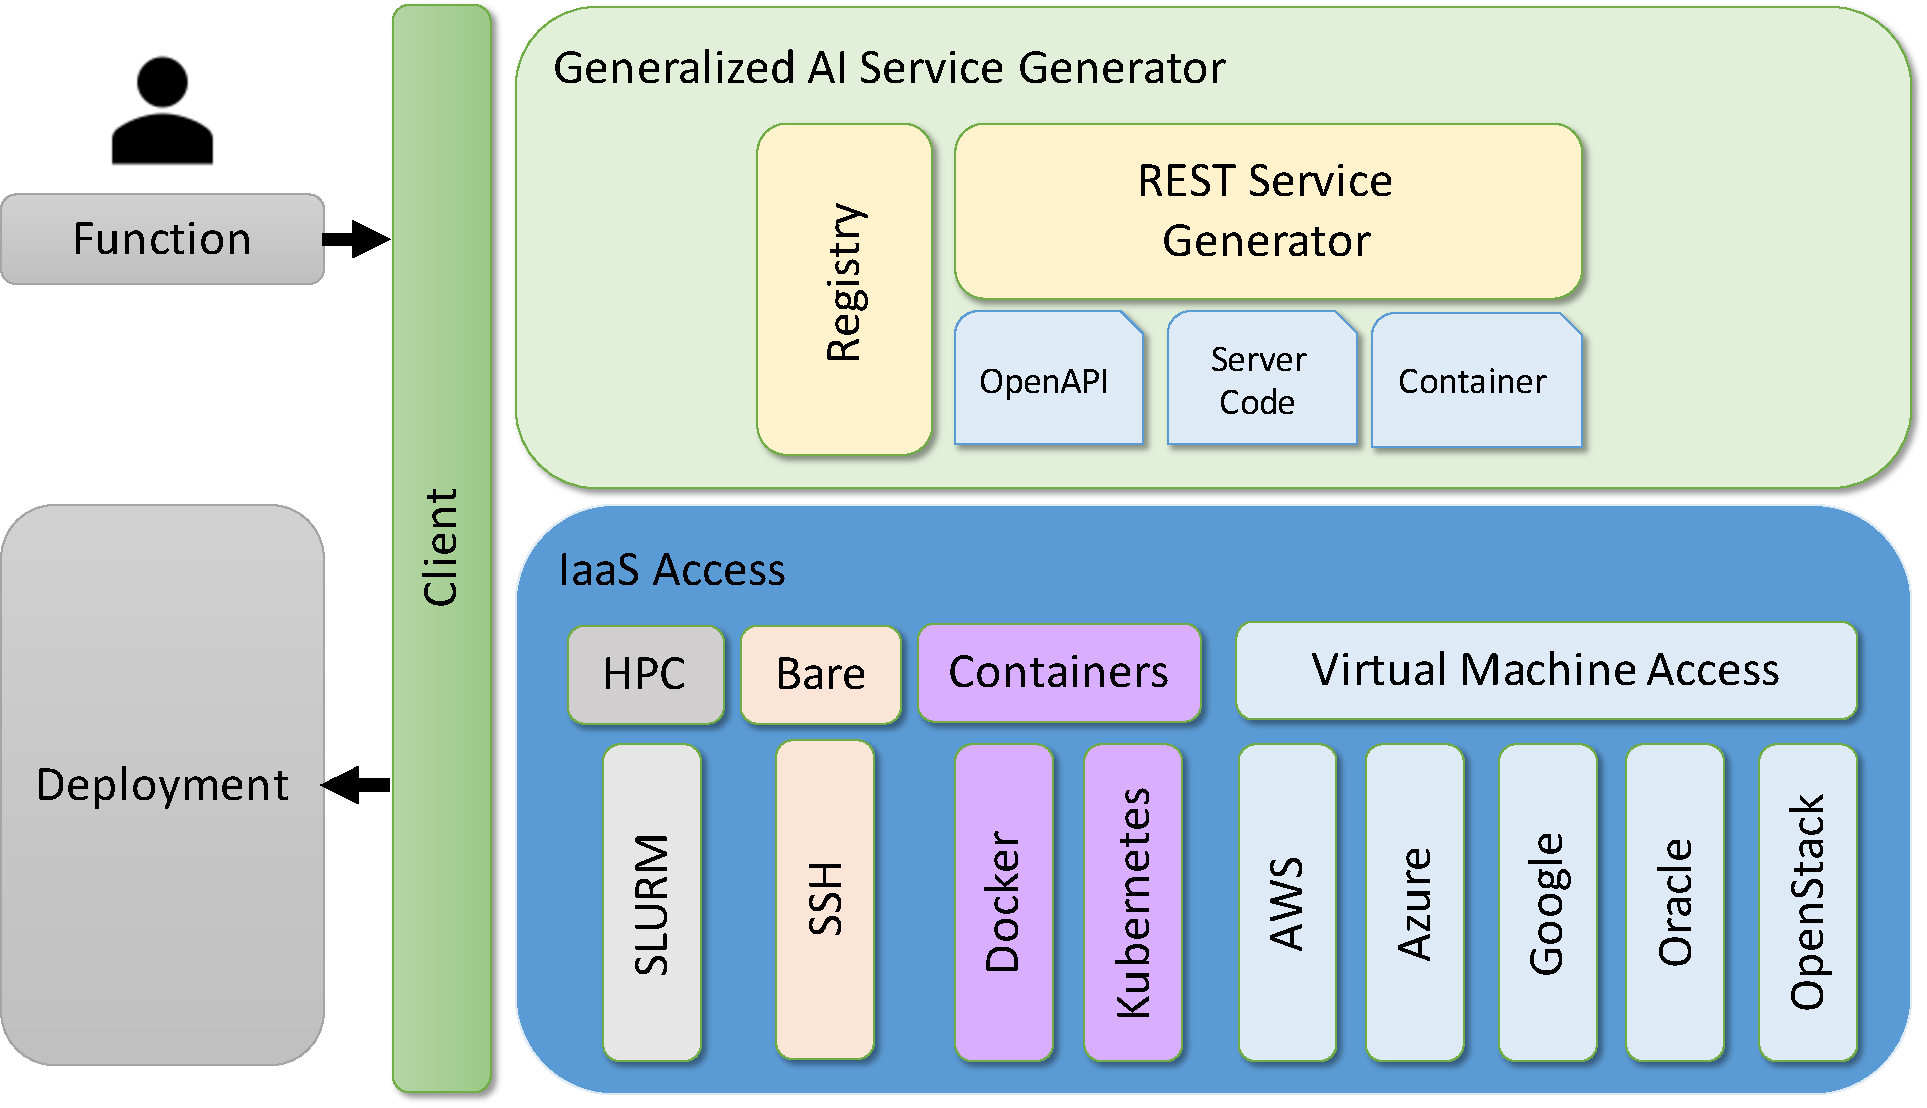
\includegraphics[width=0.7\columnwidth]{images/openapi-arch-new-2.pdf}
}{This figure shows the two layers of the Architecture. One is the IaaS Layer, the other is the openapi layer.}
\end{center}

{\em Fig 1. Layered architecture of the cloudmesh Open\-API framework.}

\bigskip
Hence, our framework allows scientists to focus on their scientific tasks exposed to well-known programming using functions and classes as input to the generator. These functions can have AI services embedded in them. Fig. 3 showcases our automated AI service workflow. 



\begin{center}
\pdftooltip{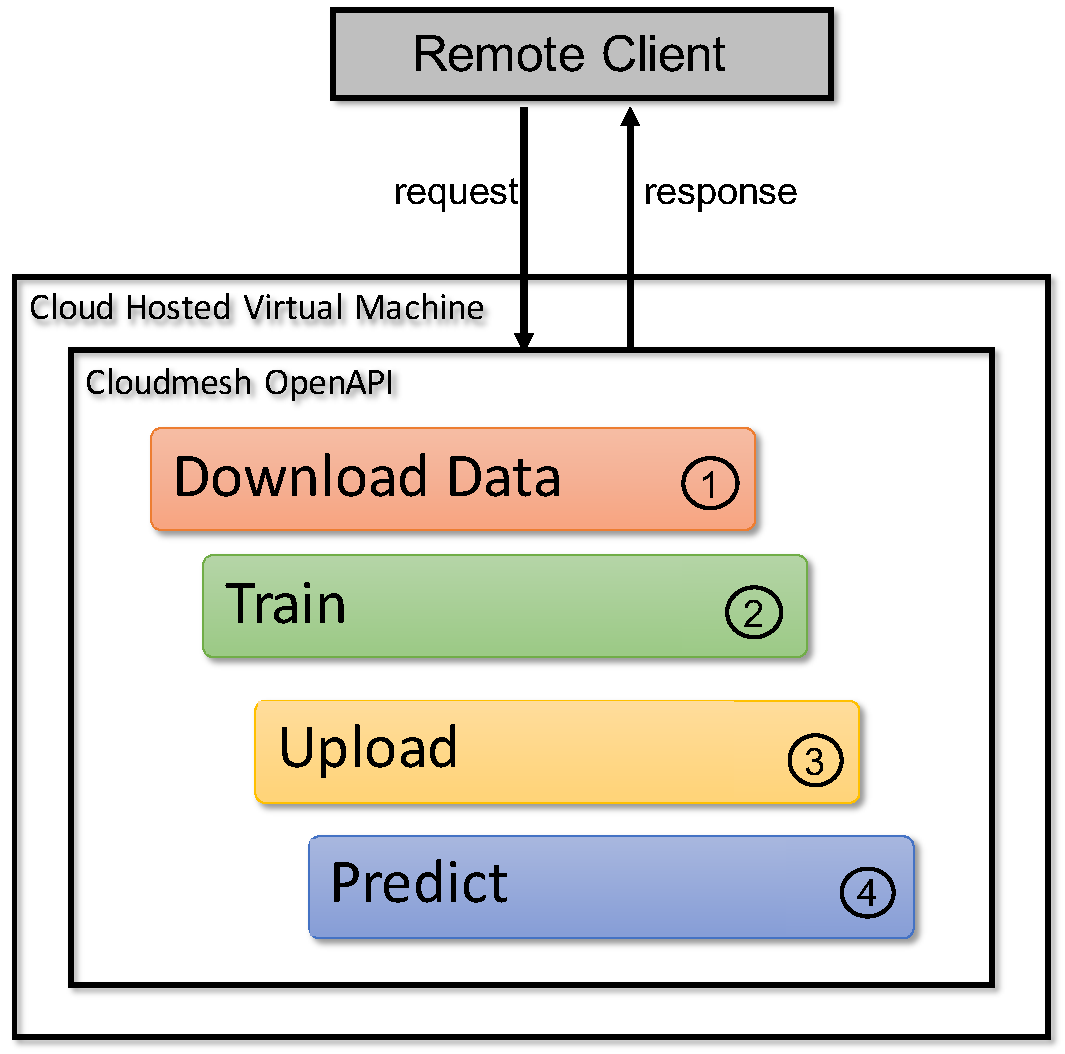
\includegraphics[width=0.5\columnwidth]{images/architecture-openapi-1.pdf}
}{This figure shows a sequence of processes between remote client, download data, train, upload, and predict.}
\end{center}

{\em Fig 2. High-level overview of the benchmark test sequence.}


\begin{center}
\pdftooltip{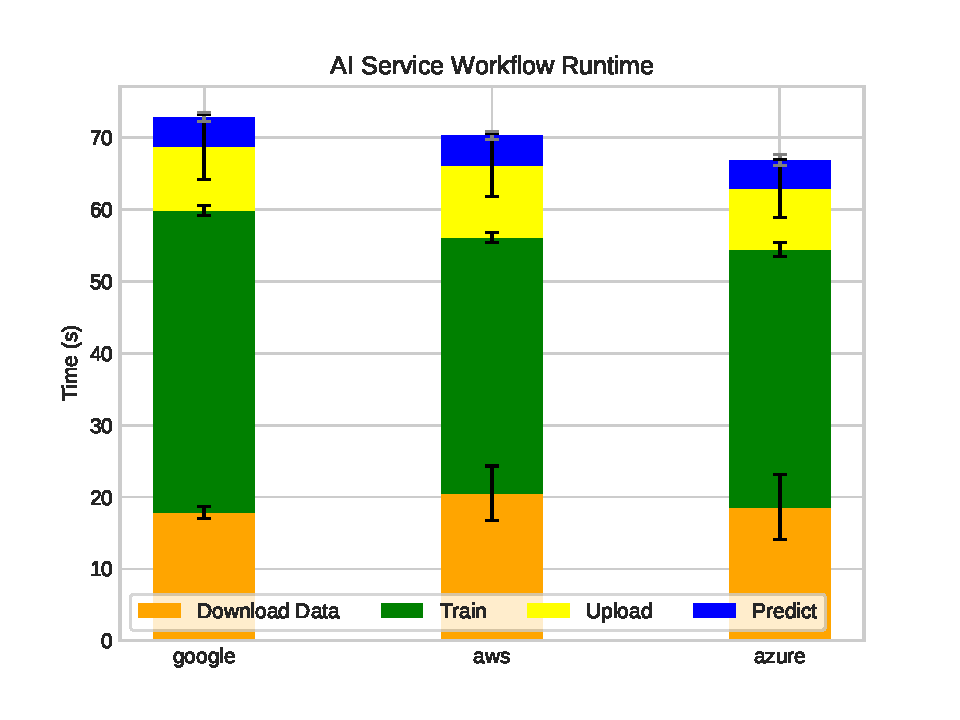
\includegraphics[width=0.6\columnwidth]{images/ai_service_workflow_runtime.pdf}
}{This figure shows the benchmark results between AWS, Azure, and Google. As the similar VMs are used the time is similar.}
\end{center}

{\em Fig 3. Comparison of the performance of Eigenface SVM algorithm on various clouds auto-generated from cloudmesh-openapi.}

\section*{Benchmark.}

We developed examples based on the reuse of Scikit-learn artificial intelligent algorithms demonstrations. These examples are then run on different cloud services to create comparative performance benchmarks. We conducted the benchmarks on 
AWS, Azure, and Google. Additional examples conducted on IoT devices and personal computers are discussed in [1]. We also compared the overhead of using the REST services [1].


\section*{Conclusion.}

In our benchmarks, we see that the cloud providers, when using similar resources and images, perform similarly (see Fig. 3). For small enough examples we find that IoT devices (such as Raspberry PI's) perform very well [1]. Due to this good performance, the PI's are very cost-effective for the examples we chose.
Future, work will include more compute-intensive tasks and additional benchmarks.

However, our most significant gain from this project is the reduction in manpower and entry barrier it takes to create and deploy our AI services. Due to the generalized approach when using python functions developers and data scientists can naturally integrate more complex tasks as well as tasks that leverage cloud-specific AI services that are uniquely offered by particular providers. GAS Generator is an open-source project, and we appreciate contributions to the project. 

\section*{Acknowledgment.} We would like to thank Lamara DeChelle Warren for initiating the contact of the UROC students so they can be part of this effort. 
We would also like to thank
B. Kegerreis,
J. Beckford,
J. Kandimalla,
P. Shaw,
I. Mishra,
F. Wang, and A. Goldfarb for developing the service generator this work is leveraging. Finally, we would like to thank the NIST NBDIF working group for their input.

\section*{References.}

[1] Using GAS for Speedy Generation of Hybrid Multi-Cloud AutoGenerated AI Services
G. von Laszewski,
A. Orlowski,
R. H. Otten,
R. Markowitz,
S. Gandhi,
A. Chai,
C. Wilson, and
G. C. Fox,
W. L. Chang
\url{https://github.com/laszewski/laszewski.github.io/raw/master/papers/vonLaszewski-openapi.pdf}

%\bibliographystyle{IEEEtran}
%\bibliography{bib/references}

\section*{Contact.} ~\\
URL: \url{https://laszewski.github.io}\\
Email: laszewski@gmail.com


\end{multicols}
\end{document}